%% taken from https://tex.stackexchange.com/questions/142660

% ***********************************************************
% ******************* PHYSICS HEADER ************************
% ***********************************************************
% Version 2
\documentclass[12pt]{article}
\usepackage{amsmath} % AMS Math Package
\usepackage{amsthm} % Theorem Formatting
\usepackage{amssymb}    % Math symbols such as \mathbb
\usepackage{graphicx} % Allows for eps images
\usepackage[dvips,letterpaper,margin=1in,bottom=0.7in]{geometry}
\usepackage{tensor}
 % Sets margins and page size
\usepackage{amsmath}
\usepackage{hyperref}
\usepackage{color}
\usepackage{listings}
\lstset{language=Python}

\definecolor{dkgreen}{rgb}{0,0.6,0}
\definecolor{gray}{rgb}{0.5,0.5,0.5}
\definecolor{mauve}{rgb}{0.58,0,0.82}
\lstset{frame=tb,
	language=Python,
	aboveskip=3mm,
	belowskip=3mm,
	showstringspaces=false,
	columns=flexible,
	basicstyle={\small\ttfamily},
	numbers=none,
	numberstyle=\tiny\color{gray},
	keywordstyle=\color{blue},
	commentstyle=\color{dkgreen},
	stringstyle=\color{mauve},
	breaklines=true,
	breakatwhitespace=true,
	tabsize=4
}

\renewcommand{\labelenumi}{(\alph{enumi})} % Use letters for enumerate
% \DeclareMathOperator{\Sample}{Sample}
\let\vaccent=\v % rename builtin command \v{} to \vaccent{}
\usepackage{enumerate}
\renewcommand{\v}[1]{\ensuremath{\mathbf{#1}}} % for vectors
\newcommand{\gv}[1]{\ensuremath{\mbox{\boldmath$ #1 $}}} 
% for vectors of Greek letters
\newcommand{\uv}[1]{\ensuremath{\mathbf{\hat{#1}}}} % for unit vector
\newcommand{\abs}[1]{\left| #1 \right|} % for absolute value
\newcommand{\avg}[1]{\left< #1 \right>} % for average
\let\underdot=\d % rename builtin command \d{} to \underdot{}
\renewcommand{\d}[2]{\frac{d #1}{d #2}} % for derivatives
\newcommand{\dd}[2]{\frac{d^2 #1}{d #2^2}} % for double derivatives
\newcommand{\pd}[2]{\frac{\partial #1}{\partial #2}} 
% for partial derivatives
\newcommand{\pdd}[2]{\frac{\partial^2 #1}{\partial #2^2}} 
% for double partial derivatives
\newcommand{\pdc}[3]{\left( \frac{\partial #1}{\partial #2}
 \right)_{#3}} % for thermodynamic partial derivatives
\newcommand{\ket}[1]{\left| #1 \right>} % for Dirac bras
\newcommand{\bra}[1]{\left< #1 \right|} % for Dirac kets
\newcommand{\braket}[2]{\left< #1 \vphantom{#2} \right|
 \left. #2 \vphantom{#1} \right>} % for Dirac brackets
\newcommand{\matrixel}[3]{\left< #1 \vphantom{#2#3} \right|
 #2 \left| #3 \vphantom{#1#2} \right>} % for Dirac matrix elements
\newcommand{\grad}[1]{\gv{\nabla} #1} % for gradient
\let\divsymb=\div % rename builtin command \div to \divsymb
\renewcommand{\div}[1]{\gv{\nabla} \cdot \v{#1}} % for divergence
\newcommand{\curl}[1]{\gv{\nabla} \times \v{#1}} % for curl
\let\baraccent=\= % rename builtin command \= to \baraccent
\renewcommand{\=}[1]{\stackrel{#1}{=}} % for putting numbers above =
\providecommand{\wave}[1]{\v{\tilde{#1}}}
\providecommand{\fr}{\frac}
\providecommand{\RR}{\mathbb{R}}
\providecommand{\NN}{\mathbb{N}}
\providecommand{\seq}{\subseteq}
\providecommand{\e}{\epsilon}

\newtheorem{prop}{Proposition}
\newtheorem{thm}{Theorem}[section]
\newtheorem{axiom}{Axiom}[section]
\newtheorem{p}{Question}[section]
\usepackage{cancel}
\newtheorem*{lem}{Lemma}
\theoremstyle{definition}
\newtheorem*{dfn}{Definition}
 \newenvironment{s}{%\small%
        \begin{trivlist} \item \textbf{Solution}. }{%
            %\hspace*{\fill} $\blacksquare$\end{trivlist}}%
			\end{trivlist}}%
% ***********************************************************
% ********************** END HEADER *************************
% ***********************************************************\texttt{}

\begin{document}
	
	{\noindent\Huge\bf  \\[0.5\baselineskip] {\fontfamily{cmr}\selectfont  Problem Set 6}         }\\[2\baselineskip] % Title
	{ {\bf \fontfamily{cmr}\selectfont Phys 589: Biostatistics}\\ {\textit{\fontfamily{cmr}\selectfont     October 17, 2018}}}~~~~~~~~~~~~~~~~~~~~~~~~~~~~~~~~~~~~~~~~~~~~~~~~~~~~~~~~~~~~~~~~~~~~~~~~~~~~~    {\large \textsc{Jonathan Monroe}} % Author name
	\\[1.4\baselineskip] 
	
	
	
	\section{Noisy sequences}
	{Opening the \textit{.FASTQ} file reveals sequenced DNA strands organized in the following format:
			\begin{enumerate}[\quad1.]
				\item ``@(identifier) [optional comments]''
				\item Sequence letters
				\item ``+ [optional description and repeat of sequence]''
				\item Quality flags
			\end{enumerate}	
			The quality flags assign an alphanumeric character to quantify the quality, $Q$. $Q$ is given by the character's ASCII decimal code, e.g. 33 for `!' and 126 (`~') for a total of 94 options. $Q$ corresponds to the occurrence probability, $p$, via $p=10^{-(Q-33)/10}$.
	}
	\begin{p} Which sequence seem noisier?
	\end{p}
	\begin{s} Sequence 3 and 6 contain a number of `/' corresponding to bottom-third quality. More quantitatively, the sum of the quality factors for these sequences seems ``statistically lower'', as in Figure  \ref{fig:qualitysequencenum}.
	\begin{figure}[h]
		\centering
		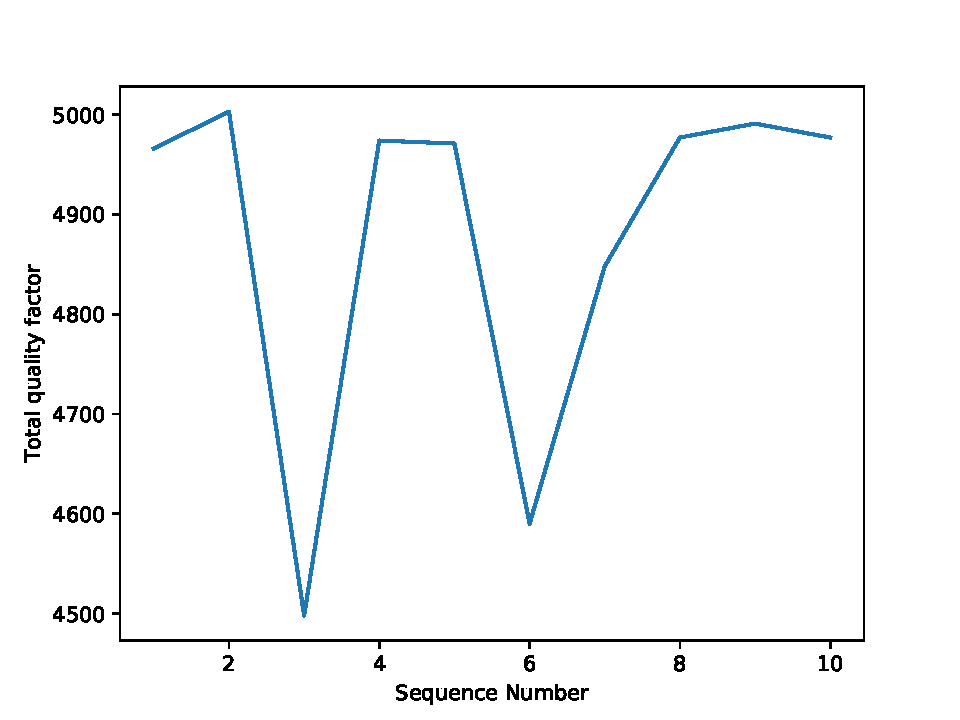
\includegraphics[width=0.4\linewidth]{figures/quality_sequenceNum}
		\caption{}
		\label{fig:qualitysequencenum}
	\end{figure}	
	\end{s}


	\section{Identification}
	Searching the National Medical Library's \textit{Basic Local Alignment Search Tool} for the first sequence indicates that it belongs to \textit{Lactobacillus salivarius}. I was surprised that so many other \textit{Lactobacillus} species fit so closely. The score metric maximizes for many of the other fits, and the \href{https://www.ncbi.nlm.nih.gov/books/NBK21106/#app8}{documentation} does not offer a clarifying definition. Nonetheless, because the \textit{ident} field maximizes for \textit{L. salivarius} and not for others I believe this is the represented organism.
	
	\section{Difference identification}
	Here we list the full sequence with highlighted differences:
	\tiny
	
	%STANDARD
GCAAGCGTTGTCCGGATTTATTGGGCGTAAAGGGAACGCAGGCGGTCTTTTAAGTCTGATGTGAAAGCCTTCGGCTTAACCGGAGTAGTG
\phantom{loremip}CATTGGAAACTGGAAGACTTGAGTGCAGAAGAGGAGAGTGGAACTC

%
%TO COMPARE
GCAAGCGTTGTCCGGATTTATTGGGCGTAAAGGGAACGCAGGCGGTCTTTTAAGTCTGATGTGAAAGCCTTCGGCTTAACCGGAGTAGTG
\phantom{loremip}CATTGGAAACTGGAAGACTTGAGTGC\color{red}G\color{black}GAAGAGGAGAGTGGAACTC

GCAAGCGTTGTCCGGATTTATTGGGCGTAAAGGGAACGCAGGCGGTCTTTTAAGTCTGATGTGAAAGCCTTCGGCTTAACCGGAGTAGTG
\phantom{loremip}CATTGGAAACTGGAAGACTTGAGTGCAGAAGAGGAGAGTGGAACTC

GCAAGCGTTGTCCGGATTTATTGGGCGTAAAGGGAACGCAGGCGGTCTTTTAAGTCTGATGTGAAAGCCTTCGGCTTAACCGGAGTAGTG
\phantom{loremip}CATTGGAAACTGGAAGACTTGAGTGC\color{red}G\color{black}GAAGAGGAGAGTGGAACTC

GCAAGCGTTGTCCGGATTTATTGGGCGTAAAGGGAACGCAGGCGGTCTTTTAAGTCTGATGTGAAAGCCTTCGGCTTAA\color{red}A\color{black}CGGAGTAGTG
\phantom{loremip}CATTGGAAACTGGAAGACTTGAGTGC\color{red}G\color{black}GAAGAGGAGAGTGGAACTC

GCAAGCGTTGTCCGGATTTATTGGG\color{red}A\color{black}GTAAAGGGAACGCAGGCGGTCTTTTAAGTCTGATGTGAAAGCCTTCGGCTTAACCGGAGTAGTG
\phantom{loremip}CATTGGAAACTGGAAGACTTGAGTGCAGAAGAGGAGAGTGGAACTC

GCAAGCGTTGTCCGGATTTATTGGGCGTAAAGGGAACGCAGGCGGTCTTTTAAGTCTGATGTGAAAGCCTTCGGCTTAACCGGAGTAGTG
\phantom{loremip}CATTGGAAACTGGAAGACTTGAGTGCAGAAGAGGAGAGTGGAACTC

GCAAGCGTT\color{red}A\color{black}TCCGGATTTATTGGGC\color{red}A\color{black}TAAAGGGAACGCAGGCGGTCTTTTAAGTCTGATGTGAAAGCCTTCGGCTTAACCGGAGTAGTG
\phantom{loremip}CATTGGAAACTGG\color{red}G\color{black}AGACTTGAGTGCAGAAGAGGAGAGTGGAACTC

GCAAGCGTTGTCCGGATTTATTGGGCGTAAAGGGAACGCAGGCGGTCTTTTAAGTCTGATGTGAAAGCCTTCGGCTTAACCGGAGTAGTG
\phantom{loremip}CATTGGAAACTGGAAGACTTGAGTGCAGAAGAGGAGAGTGGAACTC

GCAAGCGTTGTCCGGATTTATTGGGCGTAAAGGGAACGCAGGCGGTCTTTTAAGTCTGATGTGAAAGCCTTCGGCTTAACCGGAGTAGTG
\phantom{loremip}CATTGGAAACTGGAAGACTTGAGTGC\color{red}G\color{black}GAAGAGGAGAGTGGAACTC
	
	\normalsize
	We note that 4 of the sequences seem to have the same substitution error and 3 seem to have substitutions in dissimilar positions, whereas 2 others have a close, but unique error. 

	\section{Error sources}
	
	The two major sources of substitution errors in 16S data are: the Illumina sequencer itself, and a molecular machine called \underline{DNA polymerase}, used in a reaction called \linebreak\underline{Polymerase chain reaction (PCR)}, to selectively amplify the 16S-encoding DNA prior to its sequencing.
	
	\section{Error source evaluation}
	This process of DNA multiplication can include a number of differences among nucleotides. First, biological diversity clearly creates differences in DNA sequences. Second, sequencing errors can also induce nucleotide differences. Of these, errors due to contaminated specimens and nucleotide misidentification can both occur. However, only \textbf{artifacts of sequencing} (misidentification) can be flagged by the sequence itself.

	\section{Errors in sequencing}
	One can identify which sequences seem to have which type of error by evaluating the read quality of each differing nucleotide. In these comparisons quality flag ``E'' seems to be the highest achieved accuracy, and I'll assume these nucleotides are read correctly.

	\begin{enumerate}
		\item No differences
		
		\texttt{Seq 3}, \texttt{Seq 7}, and \texttt{Seq 9} match the reference (\texttt{Seq 1}).
		
		\item Real biological
		
		\texttt{Seq 2}, \texttt{Seq 4}, and \texttt{Seq 10} disagree in nucleotide number 117 with quality flag ``E'' suggesting an accurate detection of a legitimate biological difference. The repeated substitution in multiple sequences seems to suggest a biological mechanism which produces these mutations.

		\item Artifact of sample prep
		
		Likewise, \texttt{Seq 8} contains 3 separate differences from the reference, however, these are all high quality reads. Because these nucleotides are distant from each other, I suspect this sequence comes from an organism which contaminated the sample. 		
		
		\item Artifact of sequencing
		
		\texttt{Seq 6} disagrees at nucleotide number 26 with quality flag ``2''. Because this quality score is 19 points lower (on a 94 point scale), I conclude this is likely a sequencer error.		
		
		\item Artifact of sequencing \textbf{and} real biological
		
		Finally, \texttt{Seq 5} contains the same shift in nucleotide 117 with high quality read, however, it also differs in nucleotide 80. Because the latter read has low quality flag ``6'' (15 below ``E'') I conclude that this sequence has both biological diversity and sequencer error.
	\end{enumerate}

	In the end, these classifications are not air-tight. I've assumed a standard for ``perfect sequencing'' which is untested, and I have chosen arbitrary quality flag differences. More substantially, I've used plurality as a measure of biological significance which presently has no biological justification.

	Perhaps these samples are poorly produced so that the best quality flag is actually fairly mis-representative. Systematic nucleotide mis-identification would be hard to eliminate.
	To the contrary, the striking disparity between overall quality flag for \texttt{Seq 3} and it's agreement with the reference indicate that even low quality reads can give accurate sequences.
	
	\section{Eliminating uncertainty}
	A technical replicate would be a great means to check some of these hypothesis. If the same difference in nucleotide number 117 occurs with comparable frequency then this would a strong case for a biological mechanism. Moreover, repeated ``artifact of sequencing'' errors would suggest that these are instead real biological differences (especially if differences were recorded higher quality). 
	Unfortunately, ``Artifact of sample prep'' errors are more difficult to diagnose. If they are systematic issues (e.g.\ due to a dirty lab environment) contamination could persist. However, if they are sample-specific errors then they would likely be eliminated in a technical replicate.
	
	\section{Source Code}
	Here is my code:
	\lstinputlisting{dataProcessing.py}


\end{document}